\documentclass[__main__.tex]{subfiles}

\begin{document}

\qtitle{Э}{03}
Сила Ампера. Магнитное поле прямого постоянного тока. Сила взаимодействия двух коллинеарных постоянных токов.\\ 

%%
\textbf{Сила ампера}\\

\begin{wrapfigure}{L}{.3\linewidth}
	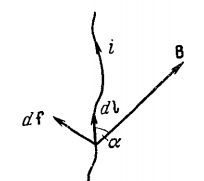
\includegraphics{e-03-amper}
	\caption{Сила Ампера}
	\label{e-03-force}
\end{wrapfigure}
Согласно закону Ампера на элемент тока $d\vec{I}$ действует в магнитном поле сила
\begin{gather}
	d\vec{f} = kid\vec{I} \times \vec{B},
	\label{e-03-amper}
\end{gather}
где $k$ - коэффициент пропорциональности,\\
$i$ - сила тока,\\
$\vec{B}$ - магнитная индукция в том месте, где помещается элемент $dI$.\\
Величина силы \ref{e-03-amper} вычисляется по формуле 
\begin{gather}
	df = kiBdl\sin{\alpha},
\end{gather}
где $\alpha$ - угол между векторами $d\vec{I}$ и $\vec{B}$. Сила направлена перпендикулярно к плоскости, в которой лежат $d\vec{I}$ и $\vec{B}$(рис.\ref{e-03-force}).\\

\textbf{Магнитное поле прямого постоянного тока}\\
\begin{wrapfigure}{l!}{.4\linewidth}
	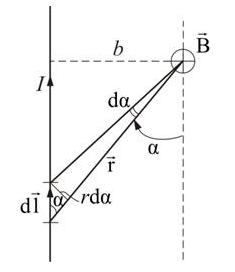
\includegraphics{e-03-field}
	\caption{Магнитное поле прямого тока}
	\label{e-03-field}
	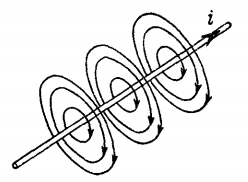
\includegraphics{e-03-circle}
	\caption{Силовые линии}
	\label{e-03-circle}
\end{wrapfigure}
Рассмотрим магнитное поле прямого тока	\ref{e-02-field}\\
Все векторы $d\vec{B}$ от произвольных элементарных участков $d\vec{l}$ имеют одинаковое направление. Поэтому сложение векторов можно заменить сложением модулей.\\
Пусть точка, в которой определяется магнитное поле, находится на расстоянии $b$ от провода. Из рис.\ref{e-02-field} видно, что:
\begin{gather}
	r = \frac{b}{\sin{\alpha}}; \hspace{0.5cm} dl = \frac{rd\alpha}{\sin{\alpha}} = \frac{bd\alpha}{\sin{\alpha}^2}
	\label{e-03-r}
\end{gather}
Подставив значения \ref{e-03-r} в закон Био-Савара-Лапласа, получим:
\begin{gather*}
	dB = \frac{\mu_0}{4\pi}\frac{Ibd\alpha\sin{\alpha}\sin{\alpha}^2}{\sin{\alpha}^2b^2} = \frac{\mu_0}{4\pi}\frac{I}{b}\sin{\alpha}d\alpha
\end{gather*}
Для конечного проводника угол $\alpha$ изменяется от $\alpha_1$ до $\alpha_2$. Тогда 
\begin{gather*}
	B = \int_{\alpha_1}^{\alpha_2}{dB} = \frac{\mu_0}{4\pi}\frac{I}{b} \int_{\alpha_1}^{\alpha_2}{\sin{\alpha}d\alpha} = \frac{\mu_0I}{4\pi b}(\cos{\alpha_1} - \cos{\alpha_2})
\end{gather*}
Для бесконечно длинного проводника $\alpha_1 = 0$, а $\alpha_2 = \pi$, тогда
\begin{gather*}
	B = \frac{\mu_0I}{2\pi b}
\end{gather*}
Линии магнитной индукции прямого тока представляют собой систему концентрических окружностей, охватывающих ток (рис. \ref{e-03-circle}).
\newpage
\textbf{Сила взаимодействия двух коллинеарных постоянных токов}\\

\begin{wrapfigure}{l!}{.4\linewidth}
	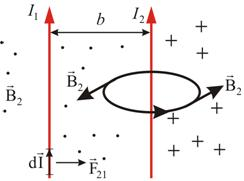
\includegraphics{e-03-colinear.jpg}
	\caption{Параллельные токи}
	\label{e-03-colinear}
\end{wrapfigure}

Пусть $b$ – расстояние между двумя параллельными, бесконечно длинными проводниками. Один из проводников $I_2$ создаёт магнитное поле, второй $I_1$ находится в этом поле(рис. \ref{e-03-colinear}).\\
$I_1$ и $I_2$ лежат в одной плоскости, синус угла между $B_2$ и прямой, на которой лежит $I_1$ $\sin{(\vec{l}, \vec{B_2})} = 1$. Тогда сила, действующая на элемент $dl$ тока $I_1$
\begin{gather}
	F_{21} = B_{2}I_{1}dl = \frac{\mu_0I_1I_2dl}{2\pi b}.
	\label{e-02-forcecol}
\end{gather}
На каждую единицу длины проводника действует сила равная $\frac{F_{21}}{dl}$. Со стороны первого проводника на второй действует точно такая же сила \ref{e-02-forcecol}.\\
Результирующая сила равна одной из этих сил. Если два проводника действуют на третий, тогда магнитные поля $\vec{B}_1$ и $\vec{B}_2$ складываются векторно.
\end{document}